\documentclass[10pt,a4paper]{article}
\usepackage[T1]{fontenc}
\usepackage[utf8]{inputenc}
\usepackage[english]{babel}
\usepackage{times,amsmath,graphicx,booktabs}
\usepackage[top=1.8cm,bottom=1.8cm,left=1.8cm,right=1.8cm]{geometry}
\usepackage{enumitem}
\setlength{\parindent}{0pt}
\setlength{\parskip}{4pt}
\setlist{nosep,leftmargin=*}
\begin{document}
\begin{center}
{\Large Network Modeling -- AY 2026/2027}\\[4pt]
{\large Homework 2 -- Composite Shaping of Zoom Outgoing Traffic}\\[5pt]
Alessandro Vulcu -- ID 2185190, University of Padua
\end{center}
\begin{abstract}
I implemented a token bucket followed by a constant-rate leaky bucket, both operating
in simulated time, using the empirical Zoom traffic source fitted in Homework 1.
A grid search selects rates and buffer capacities under loss and delay constraints.
Independent 30-minute replications confirm the chosen configuration.
The results quantify the shaper’s contribution to QoS for the estimated traffic model,
rather than the overall call quality.
\end{abstract}

\section{Source and Implementation}
In Homework 1, I selected an outgoing UDP flow from Zoom with the webcam enabled.
I use a 180 s training sample and reserve the following 120 s for validation.
Packet sizes correspond to captured Ethernet frame lengths, not multimedia payload.
I reused the training CSV file, with a clustering threshold of 1 ms and excluding
both boundary clusters. The resulting complete cycles are represented by
$(D_i,\{U_{i,k},L_{i,k}\}_{k=1}^{B_i})$: interval between cluster starts, packet
time offsets and lengths. Uniform and independent sampling of complete tuples
preserves the dependence between interval, number of packets and lengths.
The estimated mean rate is 865.95 kbit/s and the largest packet is 1\,341 B.\\

All the $B_i$ packets are emitted at the start of the cycle on separate rows with the same timestamp and the start of the next cycle is moved forward by $D_i$. 
By doing so, we preserve the distributions of the intervals between clusters, the number of packets per batch, and the lengths, while deliberately eliminating the
short offsets within clusters used in Homework 1. The source generates packets in $[0,T)$ and assigns unique consecutive IDs.\\

Then, \texttt{source.py} generates the input file, while \texttt{shaper.py} reads it and writes the output file. Both use three whitespace-separated fields: ID, timestamp in seconds, and length in bytes. Input times are the instants of generation; output times are the instants when transmission is completed.\\

The token bucket starts full, with a real-valued token balance and continuous replenishment:
\begin{equation}
    q(t+\Delta)=\min\{b,q(t)+\rho\Delta\},\qquad
t_{\rm eligible}=t+\max\{0,L_{\rm head}-q(t)\}/\rho.
\end{equation}

One token represents one byte. Only the packet at the head of the FIFO can be transmitted: the transfer consumes a number of tokens equal to its total length. The packets that exceed $b$ are dropped. If the tokens are insufficient, the packets are queued in the FIFO buffer of size $B_i$ bytes. If the space is missing, the arriving packet is dropped. Furthermore, a packet transferred to a full LBF queue is discarded, and its tokens remain consumed. \\

The LBF transmits one packet at a time for $L/\mu$ seconds without interruption. The waiting queue has capacity $B_o$. Queue capacities count the number of bytes waiting in the queue and exclude the packet currently being served. An idle transmitter can therefore accept a packet even when $B_o = 0$. \\

The simulation proceeds event by event: the clock advances directly to the next
packet arrival, the instant when enough tokens are available for the packet at
the head of the queue, or the completion of a transmission, whichever comes first.
When multiple events occur at the same time, we first handle the LBF completion,
then transfer the packets already queued in the TBF that have the necessary tokens,
and finally process new arrivals in file order.

This ensures that the FIFO order is respected, without allowing new packets to cut in front of those already waiting. After the source stops, the simulation continues until both queues are emptied. \\

The implementation passes ten automated tests covering exact timing, FIFO order,
overflow of both buffers, oversized packet rejection, input validation, source
reproduction and packet conservation. The tests also verify the TBF envelope,
the handling of small token deficits and behavior under clock shifts of up to $10^9$ s.

\clearpage

\section{QoS Constraints and Experimental Methodology}
Zoom video is interactive: waiting reduces responsiveness, delay variation increases
the buffering required by the receiver, and packet loss removes video data.
Table 1 lists six QoS constraints related solely to shaping. Offered rate and
throughput are additional descriptive metrics, not acceptance criteria.

To set the limits, I use a hypothetical frame rate of 30 fps as a reference,
corresponding to 33.3 ms per frame. A mean delay of $\leq30$ ms keeps average added
latency below one frame interval. The 50 ms limit on the 95th delay percentile
allows at most 1.5 intervals for 95\% of delivered packets, while p99 $\leq100$ ms
allows rare peaks of 3 intervals. The 30 ms limit on the 95th percentile of absolute
delay variation keeps 95\% of the changes between successive delivered-packet delays
within roughly one frame interval, reducing buffering needs during playback.
The 1\% packet-loss limit and the 99\% byte-delivery requirement prevent low delays
from masking discarded traffic or selective loss of large packets.\\

For each delivered packet $j$, the delay is $d_j=t_j^{\rm out}-t_j^{\rm in}$.
Absolute delay variation is $v_j=|d_j-d_{j-1}|$, calculated between consecutive
delivered packets, including pairs separated by lost packets. The reported jitter
is the 95th percentile of these variations. Throughput is the number of bytes
whose transmission completes in $[0,T)$ divided by $T$. Delivery fractions and
delays include the final draining of the queues. Delays apply only to delivered
packets and should therefore be interpreted alongside losses. All rates are
calculated from captured bytes.\\

I evaluate 192 configurations on the same 300 s trace, with seed 2026:
\begin{equation}
    \begin{aligned}
\rho&\in\{110,140,180,220\}\times10^3\ \mathrm{B/s},&
b&\in\{1341,4096,8192,16384\}\ \mathrm{B},\\
B_i&\in\{4096,16384\}\ \mathrm{B},&
\mu&\in\{120,220,300\}\times10^3\ \mathrm{B/s},\\
B_o&\in\{4096,16384\}\ \mathrm{B}.&&
\end{aligned}
\end{equation}

Using the same trace isolates the effects of the parameters. Of the configurations,
28 satisfy all constraints; among these, I choose the one that minimizes the
normalized resource consumption index.

\begin{equation}
    C=\frac{\rho}{10^5}+\frac{\mu}{10^5}+\frac{b+B_i+B_o}{16384}.
\end{equation}

The two reserved rates and the total capacity have unit weight after normalization.
The bucket capacity represents the burst allowance, while the buffer capacities
measure waiting space. Since each resource has a positive weight, minimization
selects a feasible, non-dominated configuration within the grid.\\

I fix the chosen configuration and run ten independent replications of 1,800 s
with seeds 3026--3035. Each replication contains approximately 196,000 packets,
or about 72,000 sampled cycles, and lasts ten times the training window. I include
the initial transient, starting with empty queues and a full token bucket.
All ten replications satisfy the constraints. Table 1 shows the mean of each
run-level statistic and the corresponding 95\% confidence interval, calculated
with Student's $t$ distribution: $\bar x\pm t_{0.975,9}s_x/\sqrt{10}$.
For quantiles, the interval refers to the mean of the individual run quantiles.
Replications are the independent statistical units, since packets are correlated.

\begin{table}[h]
\centering\small
\caption{Independent validation: means and half-widths of the 95\% confidence intervals.}
\begin{tabular}{lrr}\toprule
Metric & Proposed constraint & Mean $\pm$ half-width\\\midrule
Packet loss (\%) & $\leq 1$ & $0.169 \pm 0.014$ \\
Delivered bytes (\%) & $\geq 99$ & $99.805 \pm 0.016$ \\
Mean delay (ms) & $\leq 30$ & $16.712 \pm 0.071$ \\
Delay, p95 (ms) & $\leq 50$ & $44.889 \pm 0.294$ \\
Delay, p99 (ms) & $\leq 100$ & $68.280 \pm 0.650$ \\
Delay variation, p95 (ms) & $\leq 30$ & $18.396 \pm 0.055$ \\
Offered rate (kbit/s) & Descriptive & $865.196 \pm 1.774$ \\
Output throughput (kbit/s) & Descriptive & $863.502 \pm 1.787$ \\
\bottomrule\end{tabular}
\end{table}
\clearpage

\section{Results, Trade-offs, and Limitations}
The selected parameters are:

\begin{equation}
    (\rho,b,B_i,\mu,B_o)=(180000,4096,16384,220000,4096),\qquad C=5.50.
\end{equation}

The configuration allocates 1.44 Mbit/s to the TBF and 1.76 Mbit/s to serialization. The buffers provide a total of 20,480
B of waiting space; adding the bucket’s capacity, the total considered in the index is 24,576 B. Both rates
exceed the source’s average load—approximately 0.866 Mbit/s—because short bursts must also be handled to keep latency in check.
The initially full bucket allows a small burst to pass before enforcing the long-term rate; the transmitter
then sends the packets in sequence.

\begin{figure}[h]
\centering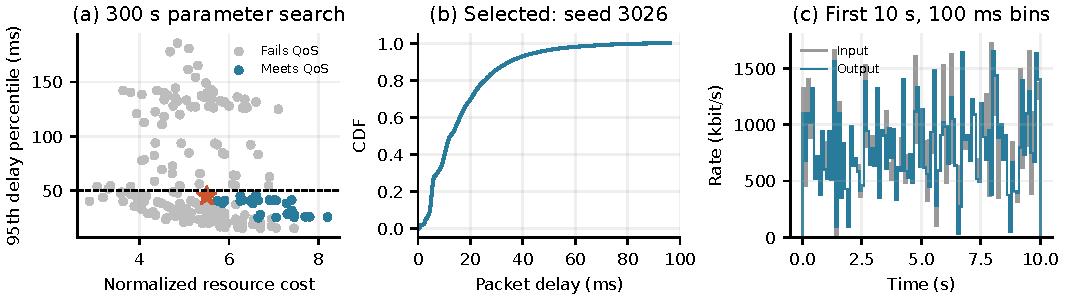
\includegraphics[width=\textwidth]{analysis/results.pdf}
\caption{Resource--delay trade-off, delivered-packet delay distribution, and input
and output rates for the selected configuration. The star marks the feasible
configuration with the lowest resource score. Rates are calculated over 100 ms
bins; packet completions may cluster near bin boundaries.}
\end{figure}

The representative replica (seed 3026) delivers 196,181 packets out of 196,556: all the 375 discarded packets occur in the input buffer. The maximum occupancy is 16,384 B in the input buffer and 4,038 B in the output wait queue. The output buffer can be small because the TBF spreads the bursts over time before passing them to the transmitter, which is faster. \\

Increasing $b$ can reduce input delay, but sends a larger burst into the output
queue. A larger $B_i$ can reduce loss at the expense of longer delays. Increasing
$B_o$ does not recover packets already dropped at the input.\\
Increasing $\rho$ reduces token wait time, while increasing $\mu$ shortens serialization and output wait time. The effect of each intervention therefore depends on the stage that limits the system.

\begin{table}[h]
\centering\small
\caption{Control cases and robustness checks, using seed 3026 for synthetic cases.}
\begin{tabular}{lrrr}\toprule
Case & Loss (\%) & p95 delay (ms) & Output (kbit/s)\\\midrule
Underprovisioned & 29.16 & 48.98 & 587.15 \\
Large buffers, low rates & 1.10 & 546.62 & 855.08 \\
Original within-batch offsets & 0.19 & 45.28 & 864.03 \\
Held-out 120 s segment & 0.04 & 31.23 & 856.88 \\
\bottomrule\end{tabular}
\end{table}

In the underprovisioned case, (90,000, 1,341, 4,096, 100,000, 4,096), delay remains
low but losses are high. The configuration with low rates and large buffers
(110,000, 8,192, 65,536, 120,000, 65,536) also violates the QoS constraints and
produces much higher delays: increasing buffer capacity alone does not compensate
for insufficient rates. Restoring the packet offsets from Homework 1 yields
results very similar to those of the representative replication. The held-out
segment of the same capture also satisfies all constraints, but this short check
does not replace the longer simulations.\\

Confidence intervals describe the variability of simulations based on the fitted
empirical source. They exclude uncertainty from the 180-second training sample,
different users or network paths, and the missing slow temporal correlation
identified in Homework 1. Independent cycle sampling loses that correlation and
overestimates some variability over 100 ms intervals. Repeating simulations does
not add new observations of real traffic.

\paragraph{Conclusion.}
The selected configuration meets all six QoS constraints in each of the ten
independent 30-minute replications and achieves the lowest resource score
($C=5.50$) among the feasible candidates in the tested grid. The control cases
show that larger buffers alone cannot compensate for insufficient rates.
These results support the selected configuration for the fitted Zoom traffic
model, under the chosen QoS budgets and resource weights.

\end{document}
